\documentclass{beamer}
\usetheme{Madrid}

\usepackage{amsmath}
\usepackage{graphicx}
\usepackage{multicol}
\usepackage{multirow}

\usepackage{tikz}
\usetikzlibrary{shapes.geometric, arrows}
% \usepackage{pgfplots}

\usepackage[justification=centering]{caption}
\usepackage{subcaption}

\usepackage{xurl}

% default path to images and other assets
\graphicspath{{../assets/}}

% disable wrapping
\tolerance=1
\emergencystretch=\maxdimen
\hyphenpenalty=10000
\hbadness=10000

% number figure caption
\setbeamertemplate{caption}[numbered]

% display bib label in references
\setbeamertemplate{bibliography item}{\insertbiblabel}
\setbeamertemplate{bibliography entry title}{}
\setbeamertemplate{bibliography entry location}{}
\setbeamertemplate{bibliography entry note}{}

% Metadata
% ------------------------
\title[MultiCut GNN]{Graph neural network for solving the minimum cost multicut problem}
\subtitle{Research seminar combinatorial image analysis}

\author{Oleh Shkalikov}

\institute[TU Dresden]{TU Dresden, Computer Science Faculty}

\date{13 June, 2023}

% ------------------------


\tikzstyle{main_node} = [circle, minimum width=1cm,text centered, draw=black, fill=red!30]
\tikzstyle{neigh_node} = [circle, minimum width=1cm,text centered, draw=black, fill=green!30]
\tikzstyle{node} = [circle, minimum width=1cm,text centered, draw=black, fill=cyan!30]
\tikzstyle{arrow} = [thick,->,>=stealth]

\begin{document}

\frame{\titlepage}

\begin{frame}
    \frametitle{Agenda}
    \tableofcontents
\end{frame}

\section{The multicut problem and introduction to GNN}

\begin{frame}
    \frametitle{Minimum Cost MultiCut Problem}

    For the given graph $G = (V, E)$ and an associated cost
    function $w: E \to \mathbb{R}$, the multicut problem is

    \begin{alignat*}{2}
        \min_{y \in \{0, 1\}^E} \quad &
        c(y) = \sum\limits_{e \in E} w_e y_e                                            \\
        \text{subject to:}      \quad &
        y_e \leq \sum\limits_{e' \in C \setminus \{e\}} y_{e'}                          \\
                                      & \forall C \in \text{cycles}(G), \forall e \in C
    \end{alignat*}

    \begin{alertblock}{Complexity}
        The problem of finding the optimal solution for this ILP
        is NP-hard problem. Moreover, the number of constraints grows
        exponentially.
    \end{alertblock}

\end{frame}

\begin{frame}
    \frametitle{Graph Neural Network}

    For the given update function $\gamma$, message $\phi$, and
    commutative aggregation operation $\bigotimes$, the update rule for every
    node $i$ at step $t$ with node feature vector $\mathbf{x}$ and
    edge feature vector $\mathbf{e}$ (optional) is
    \[
        \mathbf{x}_i^{(t+1)} = \gamma^{(t)} \left(\mathbf{x}_i^{(t)},
        \bigotimes_{j \in \mathcal{N}(i)} \phi^{(t)} \left(\mathbf{x}^{(t)}_i,
        \mathbf{x}^{(t)}_j, \mathbf{e^{(t)}}_{j, i} \right) \right)
    \]

    \begin{figure}
        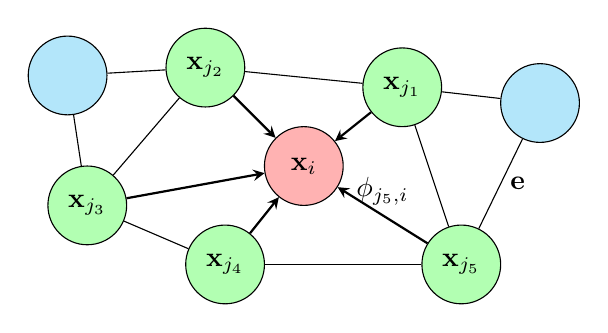
\begin{tikzpicture}[node distance=1.25cm]
            \node(main) [main_node] {$\mathbf{x}_i$};
            \node(neigh1) [neigh_node, right of=main, yshift=1cm] {$\mathbf{x}_{j_1}$};
            \node(neigh2) [neigh_node, left of=main, yshift=1.25cm] {$\mathbf{x}_{j_2}$};
            \node(neigh3) [neigh_node, left of=main, xshift=-1.5cm, yshift=-0.5cm] {$\mathbf{x}_{j_3}$};
            \node(neigh4) [neigh_node, below of=main, xshift=-1cm] {$\mathbf{x}_{j_4}$};
            \node(neigh5) [neigh_node, below of=main, xshift=2cm] {$\mathbf{x}_{j_5}$};

            \node(node1) [node, right of=neigh1, xshift=0.5cm, yshift=-0.2cm] {};
            \node(node2) [node, left of=neigh2, xshift=-0.5cm, yshift=-0.1cm] {};

            \draw[arrow] (neigh1) -- (main);
            \draw[arrow] (neigh2) -- (main);
            \draw[arrow] (neigh3) -- (main);
            \draw[arrow] (neigh4) -- (main);
            \draw[arrow] (neigh5) -- node[above]{$\phi_{j_5, i}$} (main);

            \draw (neigh1) -- (neigh2);
            \draw (neigh1) -- (neigh5);
            \draw (neigh2) -- (neigh3);
            \draw (neigh3) -- (neigh4);
            \draw (neigh4) -- (neigh5);
            \draw (neigh1) -- (node1);
            \draw (neigh5) -- node[right]{$\mathbf{e}$} (node1);
            \draw (neigh2) -- (node2);
            \draw (neigh3) -- (node2);
        \end{tikzpicture}
        \caption{Illustration of the message passing scheme}
    \end{figure}

\end{frame}

\begin{frame}
    \frametitle{Laplacian and Discrete Fourier Transform}
    The discrete fourier transform can be represented as a matrix:
    \[
        U = \begin{pmatrix}
            u_0(0)   & u_1(0)   & \dots  & u_{N-1}(0)   \\
            u_0(1)   & u_1(1)   & \dots  & u_{N-1}(1)   \\
            \vdots   & \vdots   & \ddots & \vdots       \\
            u_0(N-1) & u_1(N-1) & \dots  & u_{N-1}(N-1)
        \end{pmatrix}
    \]
    where
    \[
        u_n(x) = \cos\left(2 \pi \frac{n}{N} x \right) -
        i \sin\left(2 \pi \frac{n}{N} x \right)
    \]

    At the same time these $u_n$ are eigenvectors of the
    Laplacian operator:
    \[
        \Delta u_n(x) = \left( -4 \pi \frac{n^2}{N^2} \right) u_n(x)
    \]

\end{frame}

\begin{frame}
    \frametitle{Graph Convolutional Network}

    For the given adjacency matrix $A$ and degree matrix $D$ the
    graph laplacian is the following:
    \[
        L = I_N - D^{-\frac{1}{2}} A D^{-\frac{1}{2}} = U \Lambda U^T
    \]

    Thus, the convolution can be computed:
    \[
        g_{\theta} \star \mathbf{x} = U \hat{g}_{\theta} U^T \mathbf{x}
    \]

    Approximated form \cite{kipf2016semi} after renormalization trick as a message passing:
    \[
        \mathbf{x}_i^{(t+1)} =
        \sum_{j \in \mathcal{N}(i) \cup \{ i \}}
        \frac{\theta \mathbf{x}_j^{(t)}}
        {\sqrt{\deg(i)} \sqrt{\deg(j)}}
    \]

\end{frame}

\section{GNN approaches for multicuts}

\subsection{Supervised learning}

\begin{frame}
    \frametitle{GNN MultiCut Pipeline}

    \begin{enumerate}
        \item Compute initial node features \cite{jung2022learning}
              \[
                  \mathbf{x}_i = \left(
                  \sum\limits_{j \in \mathcal{N}^{+}(i)} w_{ij},
                  \sum\limits_{j \in \mathcal{N}^{-}(i)} w_{ij}
                  \right)
              \]
        \item Apply GNN
        \item Classify edge based on node embeddings (e.g. with MLP)
        \item Enforce cycle consistency
    \end{enumerate}

    \begin{figure}
        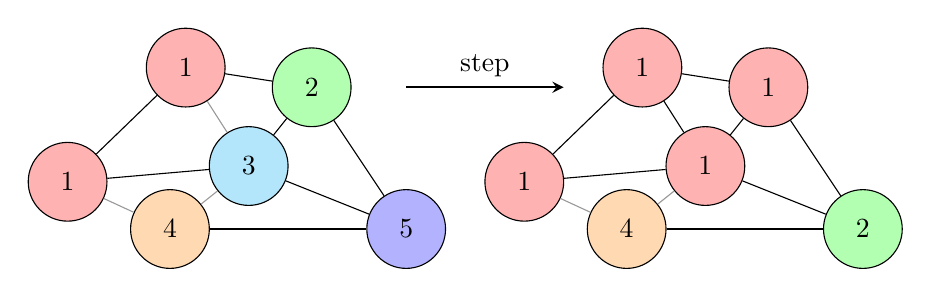
\begin{tikzpicture}[node distance=0.8cm]
            \node(root) [node] {3};
            \node(node1) [node, fill=green!30, right of=root, yshift=1cm] {2};
            \node(node2) [node, fill=red!30, left of=root, yshift=1.25cm] {1};
            \node(node3) [node, fill=red!30, left of=root, xshift=-1.5cm, yshift=-0.2cm] {1};
            \node(node4) [node, fill=orange!30, below of=root, xshift=-1cm] {4};
            \node(node5) [node, fill=blue!30, below of=root, xshift=2cm] {5};

            \node(root2) [node, fill=red!30, right of=root, xshift=5cm] {1};
            \node(node21) [node, fill=red!30, right of=root2, yshift=1cm] {1};
            \node(node22) [node, fill=red!30, left of=root2, yshift=1.25cm] {1};
            \node(node23) [node, fill=red!30, left of=root2, xshift=-1.5cm, yshift=-0.2cm] {1};
            \node(node24) [node, fill=orange!30, below of=root2, xshift=-1cm] {4};
            \node(node25) [node, fill=green!30, below of=root2, xshift=2cm] {2};

            \draw (node1) -- (root);
            \draw[color=gray!80] (node2) -- (root);
            \draw (node3) -- (root);
            \draw[color=gray!80] (node4) -- (root);
            \draw (node5) -- (root);

            \draw (node1) -- (node2);
            \draw (node1) -- (node5);
            \draw (node2) -- (node3);
            \draw[color=gray!80] (node3) -- (node4);
            \draw (node4) -- (node5);

            \draw[arrow] (2, 1) -- node[above]{step} (4, 1);

            \draw (node21) -- (root2);
            \draw[color=black] (node22) -- (root2);
            \draw (node23) -- (root2);
            \draw[color=gray!80] (node24) -- (root2);
            \draw (node25) -- (root2);

            \draw (node21) -- (node22);
            \draw (node21) -- (node25);
            \draw (node22) -- (node23);
            \draw[color=gray!80] (node23) -- (node24);
            \draw (node24) -- (node25);
        \end{tikzpicture}
        \caption{Postprocessing as a message passing}
    \end{figure}

\end{frame}

\begin{frame}
    \frametitle{Edge-Weighted GCN \cite{jung2022learning}}

    \begin{block}{Limitation of the classic CGN}
        The original CGN can not handle real value weights, so we need to augment this
        approach for out task.
    \end{block}

    Signed normalized graph Laplacian and
    corresponding message passing (here $\overline{\deg}(i) = \sum\limits_{j \in \mathcal{N}(i)} |w_{ij}|$):
    \[
        \mathbf{x}_i^{(t+1)} = \gamma_{\theta} \left(
        \mathbf{x^{(t)}_i} +
        \sum_{j \in \mathcal{N}(i)}
        \frac{w_{ij} \mathbf{x}_j^{(t)}}
        {\sqrt{\overline{\deg}(i)} \sqrt{\overline{\deg}(j)}}
        \right)
    \]

    The loss function consist 2 part:
    \[
        \mathcal{L} = \mathcal{L}_{BCE} + \alpha \overbrace{
            \sum\limits_{C \in cc{G, l}} \sum\limits_{e \in C} \hat{y}_e
            \prod\limits_{e' \in C \setminus \{e\}} (1 - \hat{y}_{e'})
        }^{\text{Cycle consistency loss}}
    \]

\end{frame}

\begin{frame}
    \frametitle{Evaluation Results}

    The model with 20 layers, cycle length parameter for CCL is $8$,
    node representation dimensionality is 128 and edge classifier 2-layer
    MLP with 256 hidden dimension, trained on artificially generated RandomMP dataset
    shows the following result \cite{jung2022learning}.

    \begin{table}
        \scalebox{0.75}
        {
            \begin{tabular}{|c|*{6}{c}|cc|}
                \hline
                \multirow{2}{*}{\textbf{Solver}}    & \multicolumn{6}{c|}{\textbf{Test Datasets}} & \multicolumn{2}{c|}{\textbf{Runtime [s]}}                                                                                                       \\
                                                    & IrisMP                                      & RndMP                                     & BSDS300 & CREMI  & Knott                                                   & h.mean & fwd & total   \\
                \hline
                \hline
                WGCN                                & 0.9762                                      & 0.9041                                    & 0.9204  & 0.8440 & 0.7870                                                  & 0.8815 & 0.9 & 4.8     \\
                \hline
                LR                                  & 0.8035                                      & 0.3938                                    & 0.7958  & 0.9260 & 0.7335                                                  & 0.6681 &     & N/A     \\
                MLP                                 & 0.8985                                      & 0.3099                                    & 0.6804  & 0.4845 & 0.1517                                                  & 0.3457 &     & N/A     \\
                \hline
                GAEC                                & 0.9836                                      & 0.9780                                    & 0.9997  & 0.9958 & 0.9968                                                  & 0.9907 &     & 23.2    \\
                TB GAEC\footnote{Time bounded GAEC} & 0.3642                                      & 0.0034                                    & 0.0000  & 0.1516 & 0.0000                                                  & 0.0000 &     & 6.3     \\
                LP solver\footnote{Branch \& Cut}   & 0.9882                                      & 0.9525                                    & 0.9979  & 0.9998 & OOT\footnote{Out of time: no termination within 24 Hrs} & -      &     & 31918.8 \\
                ILP solver                          & 1.0000                                      & 1.0000                                    & 1.0000  & 1.0000 & 1.0000                                                  & 1.0000 &     & 24361.2 \\
                \hline
            \end{tabular}
        }
        \caption{The values of optimal objective ratio for proposed
            GNN, simple linear regression / MLP trained on the input features
            and classic solvers.}
    \end{table}

\end{frame}

\begin{frame}
    \frametitle{Scaling Study}

    \begin{block}{Runtime}
        Graph neural network approach significantly outperform the
        classical approach in terms of runtime, but in the same time
        shows a lit bit worse objective value.
    \end{block}

    \begin{table}
        \scalebox{0.7}
        {
            \begin{tabular}{|c|*{8}{c|}}
                \hline
                \multirow{2}{*}{\textbf{Nodes}} & \multicolumn{2}{c|}{\textbf{GAEC}} & \multicolumn{2}{c|}{\textbf{LP}} & \multicolumn{2}{c|}{\textbf{ILP}} & \multicolumn{2}{c|}{\textbf{WGCN}}                                                          \\
                                                & [ms]                               & Objective                        & [ms]                              & Objective                          & [ms]          & Objective    & [ms]        & Objective \\
                \hline
                \hline
                $10^1$                          & \textbf{0 }                        & -29                              & 6                                 & -24                                & 11            & -30          & 29          & -29       \\
                $10^2$                          & \textbf{4 }                        & -327                             & 191                               & -246                               & 273           & -330         & 26          & -276      \\
                $10^3$                          & \textbf{24}                        & -3051                            & 6585                              & -2970                              & 1299          & -3093        & 29          & -2643     \\
                $10^4$                          & 228                                & -32 264                          & 688 851                           & -31531                             & 18604         & -32682       & \textbf{78} & -27 552   \\
                $10^5$                          & 2534                               & -323 189                         & \multicolumn{2}{c|}{OOT}          & 2 171 134                          & -328 224      & \textbf{557} & -269 122                \\
                $10^6$                          & 35 181                             & -3 401 783                       & \multicolumn{2}{c|}{OOT}          & \multicolumn{2}{c|}{OOT}           & \textbf{8713} & -2 182 589                             \\
                \hline
            \end{tabular}
        }
        \caption{Runtime and objective values over different approaches for
            different graph sizes}
    \end{table}

\end{frame}

\begin{frame}
    \frametitle{Learning Node Embedding: Motivation}

    \begin{figure}
        \begin{subfigure}{0.5\linewidth}
            \centering
            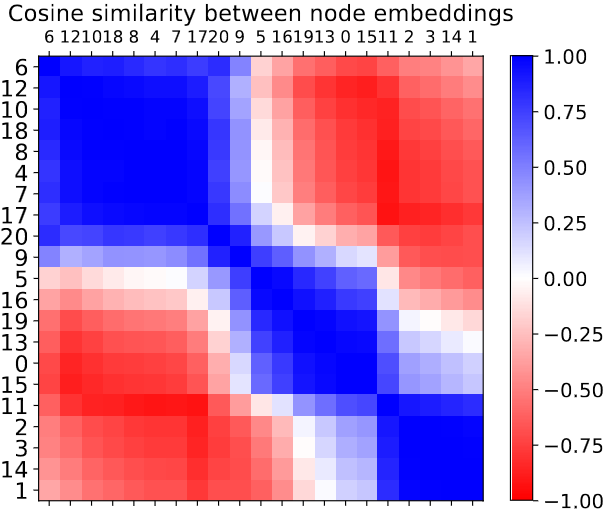
\includegraphics[height=0.53\textwidth]{emb1.png}
        \end{subfigure}
        \begin{subfigure}{0.49\linewidth}
            \centering
            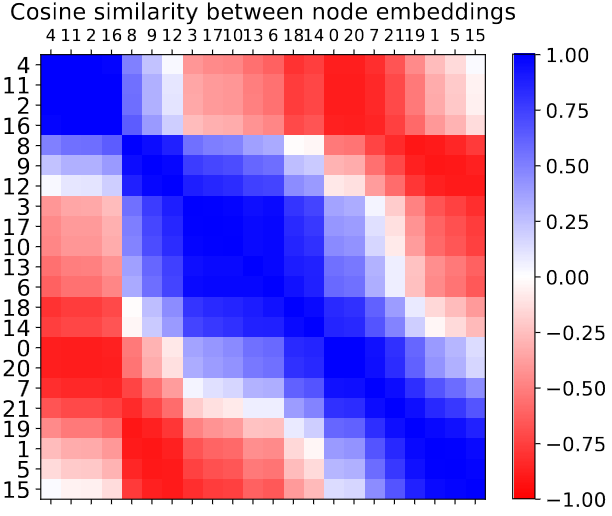
\includegraphics[height=0.53\textwidth]{emb2.png}
        \end{subfigure}
        \begin{subfigure}{0.5\linewidth}
            \centering
            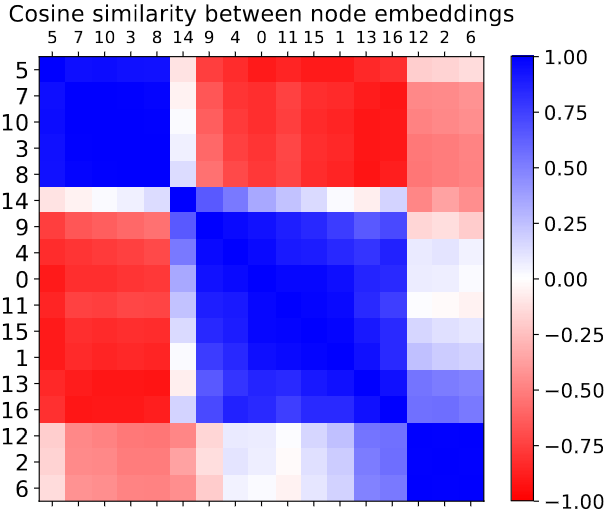
\includegraphics[height=0.53\textwidth]{emb3.png}
        \end{subfigure}
        \begin{subfigure}{0.49\linewidth}
            \centering
            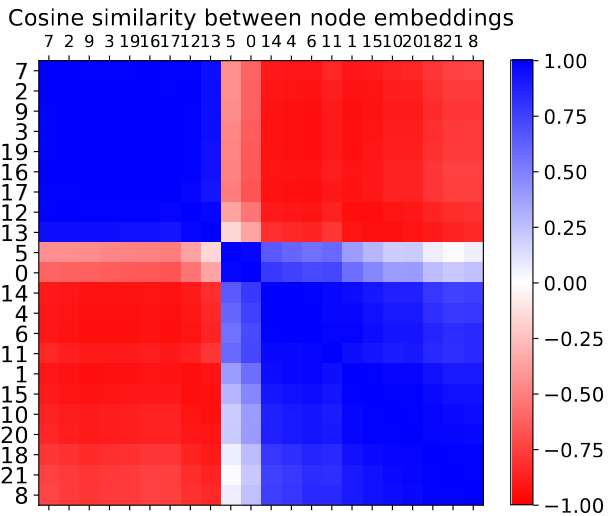
\includegraphics[height=0.53\textwidth]{emb4.png}
        \end{subfigure}
        \caption{Cosine similarities for the node embeddings
            computed for samples from the IrisMP dataset.
            Source: \cite{jung2022learning}}
    \end{figure}

\end{frame}

\begin{frame}
    \frametitle{Learning Node Embedding}

    \begin{block}{Orthogonal embeddings}
        We've seen that it is possible to learn the orthogonal
        embeddings with BCE loss,
        let's try to add / replace specific term to loss
        to ensure it. Thus we will be able to replace MLP classifier with
        scalar product calculation.
    \end{block}
    In a paper \cite{chen2019instance} on image instance segmentation
    authors proposed the following approach (here adapted to graphs):
    \[
        \mathcal{L}_{emb} =
        \lambda_1 \sum\limits_{e_{ij} \in y^{-1}(0)} \left(1 - |\cos \langle \mathbf{x}_i, \mathbf{x}_j \rangle| \right) +
        \lambda_2 \sum\limits_{e_{ij} \in y^{-1}(1)} |\cos \langle \mathbf{x}_i, \mathbf{x}_j \rangle|
    \]

    We can try to improve cycle consistency by using kernel trick ($d \geq 1$):
    \begin{multline*}
        \mathbb{P}_U \left(
        \langle \mathbf{x}_{i}, \mathbf{x}_{k} \rangle > t
        \Big|
        \langle \mathbf{x}_{i}, \mathbf{x}_{j} \rangle > t,
        \langle \mathbf{x}_{j}, \mathbf{x}_{k} \rangle > t
        \right) \leq \\
        \mathbb{P}_U \left(
        \langle \mathbf{x}_{i}, \mathbf{x}_{k} \rangle^{\textcolor{gray}{d}} > t
        \Big|
        \langle \mathbf{x}_{i}, \mathbf{x}_{j} \rangle^d > t,
        \langle \mathbf{x}_{j}, \mathbf{x}_{k} \rangle^d > t
        \right)
    \end{multline*}

\end{frame}

\begin{frame}
    \frametitle{Relaxed Cycle Consistency Loss}

\end{frame}

\begin{frame}
    \frametitle{Edge Weight Embedding}



\end{frame}

\subsection{Unsupervised learning}

\begin{frame}
    \frametitle{MultiCut Cost Loss}

\end{frame}

\subsection{Self-prior learning}

\begin{frame}
    \frametitle{Overfit Is All You Need}



\end{frame}

\section*{References}

\begin{frame}[allowframebreaks]
    \frametitle{References}

    \bibliographystyle{apalike}
    \bibliography{../references.bib}
\end{frame}

\end{document}